
%%% main document {{{

\documentclass[
a4paper,     %% defines the paper size: a4paper (default), a5paper, letterpaper, ...
% landscape,   %% sets the orientation to landscape
% twoside,     %% changes to a two-page-layout (alternatively: oneside)
% twocolumn,   %% changes to a two-column-layout
 headsepline, %% add a horizontal line below the column title
% footsepline, %% add a horizontal line above the page footer
% titlepage,   %% only the titlepage (using titlepage-environment) appears on the first page (alternatively: notitlepage)
% parskip,     %% insert an empty line between two paragraphs (alternatively: halfparskip, ...)
% leqno,       %% equation numbers left (instead of right)
% fleqn,       %% equation left-justified (instead of centered)
% tablecaptionabove, %% captions of tables are above the tables (alternatively: tablecaptionbelow)
% draft,       %% produce only a draft version (mark lines that need manual edition and don't show graphics)
% 10pt         %% set default font size to 10 point
11pt         %% set default font size to 11 point
% 12pt         %% set default font size to 12 point
]{scrartcl}  %% article, see KOMA documentation (scrguide.dvi)



%%%%%%%%%%%%%%%%%%%%%%%%%%%%%%%%%%%%%%%%%%%%%%%%%%%%%%%%%%%%%%%%%%%%%%%%%%%%%%%%
%%%
%%% packages
%%%

%%%
%%% encoding and language set
%%%

%%% ngerman: language set to new-german
\usepackage{ngerman}

%%% babel: language set (can cause some conflicts with package ngerman)
%%%        use it only for multi-language documents or non-german ones
%\usepackage[ngerman]{babel}

%%% inputenc: coding of german special characters
\usepackage[utf8]{inputenc}

%%% fontenc, ae, aecompl: coding of characters in PDF documents
\usepackage[T1]{fontenc}
\usepackage{ae,aecompl}

%%%
%%% technical packages
%%%

%%% amsmath, amssymb, amstext: support for mathematics
%\usepackage{amsmath,amssymb,amstext}

%%% psfrag: replace PostScript fonts
\usepackage{psfrag}

%%% listings: include programming code
%\usepackage{listings}

%%% units: technical units
\usepackage{units}

%%% tiefgestellte zahlen
\usepackage{subscript}

%%% mathefoo
\usepackage{amsmath}


\usepackage{xcolor}
% TikZ-Bibliotheken
\usepackage{tikz}
 \usetikzlibrary{backgrounds}
 \usetikzlibrary{matrix}
 \usetikzlibrary{circuits.ee.IEC}
 \usetikzlibrary{positioning}
 
 
%Hintergrundstyle - optional
\tikzstyle{background rectangle}=
  [thick,draw=\lightgray, fill=white!99!black, rounded corners]
 
%Volt- und Amperemeter festlegen:
\tikzset{circuit declare symbol = ammeter}
\tikzset{set ammeter graphic ={draw,generic circle IEC, minimum size=5mm,info=center:A}}
\tikzset{circuit declare symbol = voltmeter}
\tikzset{set voltmeter graphic ={draw,generic circle IEC, minimum size=5mm,info=center:V}}
\tikzset{circuit declare symbol = generator}
\tikzset{set generator graphic ={draw,rectangle ee, minimum size=5mm,info=center:G}}
% Spannungs und Strompfeile
\tikzset{
  Pfeil/.style={thick,shorten >=#1,shorten <=#1,->}, % für Peile
  UPfeil/.style={blue,Pfeil=#1,font={\sffamily\itshape}},% für Spannungspfeile
  IPfeil/.style={red,Pfeil=#1,font={\ttfamily\itshape}} % für Strompfeile
}


%Boxen
\usepackage{empheq}
 
% Command "alignedbox{}{}" for a box within an align environment
% Source: http://www.latex-community.org/forum/viewtopic.php?f=46&t=8144
\newlength\dlf  % Define a new measure, dlf
\newcommand\alignedbox[2]{
% Argument #1 = before & if there were no box (lhs)
% Argument #2 = after & if there were no box (rhs)
&  % Alignment sign of the line
{
\settowidth\dlf{$\displaystyle #1$}  
    % The width of \dlf is the width of the lhs, with a displaystyle font
\addtolength\dlf{\fboxsep+\fboxrule}  
    % Add to it the distance to the box, and the width of the line of the box
\hspace{-\dlf}  
    % Move everything dlf units to the left, so that & #1 #2 is aligned under #1 & #2
\boxed{#1 #2}
    % Put a box around lhs and rhs
}
}

%%%
%%% layout
%%%

%%% scrpage2: KOMA heading and footer
%%% Note: if you don't use this package, please remove 
%%%       \pagestyle{scrheadings} and corresponding settings
%%%       below too.
\usepackage[automark]{scrpage2}


%%%
%%% PDF
%%%

\usepackage{ifpdf}

%%% Should be LAST usepackage-call!
%%% For docu on that, see reference on package ``hyperref''
\ifpdf%   (definitions for using pdflatex instead of latex)

  %%% graphicx: support for graphics
  %\usepackage[pdftex]{graphicx}

  \pdfcompresslevel=9

  %%% hyperref (hyperlinks in PDF): for more options or more detailed
  %%%          explanations, see the documentation of the hyperref-package
  \usepackage[%
    %%% general options
    pdftex=true,      %% sets up hyperref for use with the pdftex program
    %plainpages=false, %% set it to false, if pdflatex complains: ``destination with same identifier already exists''
    %
    %%% extension options
    backref,      %% adds a backlink text to the end of each item in the bibliography
    pagebackref=false, %% if true, creates backward references as a list of page numbers in the bibliography
    colorlinks=true,   %% turn on colored links (true is better for on-screen reading, false is better for printout versions)
    %
    %%% PDF-specific display options
    bookmarks=true,          %% if true, generate PDF bookmarks (requires two passes of pdflatex)
    bookmarksopen=false,     %% if true, show all PDF bookmarks expanded
    bookmarksnumbered=false, %% if true, add the section numbers to the bookmarks
    %pdfstartpage={1},        %% determines, on which page the PDF file is opened
    pdfpagemode=None         %% None, UseOutlines (=show bookmarks), UseThumbs (show thumbnails), FullScreen
  ]{hyperref}


  %%% provide all graphics (also) in this format, so you don't have
  %%% to add the file extensions to the \includegraphics-command
  %%% and/or you don't have to distinguish between generating
  %%% dvi/ps (through latex) and pdf (through pdflatex)
  \DeclareGraphicsExtensions{.pdf}

\else %else   (definitions for using latex instead of pdflatex)

  \usepackage[dvips]{graphicx}

  \DeclareGraphicsExtensions{.eps}

  \usepackage[%
    dvips,           %% sets up hyperref for use with the dvips driver
    colorlinks=false %% better for printout version; almost every hyperref-extension is eliminated by using dvips
  ]{hyperref}

\fi


%%% sets the PDF-Information options
%%% (see fields in Acrobat Reader: ``File -> Document properties -> Summary'')
%%% Note: this method is better than as options of the hyperref-package (options are expanded correctly)
\hypersetup{
  pdftitle={}, %%
  pdfauthor={}, %%
  pdfsubject={}, %%
  pdfcreator={Accomplished with LaTeX2e and pdfLaTeX with hyperref-package.}, %% 
  pdfproducer={}, %%
  pdfkeywords={} %%
}


%%%%%%%%%%%%%%%%%%%%%%%%%%%%%%%%%%%%%%%%%%%%%%%%%%%%%%%%%%%%%%%%%%%%%%%%%%%%%%%%
%%%
%%% user defined commands
%%%

%%% \mygraphics{}{}{}
%% usage:   \mygraphics{width}{filename_without_extension}{caption}
%% example: \mygraphics{0.7\textwidth}{rolling_grandma}{This is my grandmother on inlinescates}
%% requires: package graphicx
%% provides: including centered pictures/graphics with a boldfaced caption below
%% 
\newcommand{\mygraphics}[3]{
  \begin{center}
    \includegraphics[width=#1, keepaspectratio=true]{#2} \\
    \textbf{#3}
  \end{center}
}

%%%%%%%%%%%%%%%%%%%%%%%%%%%%%%%%%%%%%%%%%%%%%%%%%%%%%%%%%%%%%%%%%%%%%%%%%%%%%%%%
%%%
%%% define the titlepage
%%%

% \subject{}   %% subject which appears above titlehead
% \titlehead{} %% special heading for the titlepage

%%% title
\title{Messbericht \\ Anpassung}

%%% author(s)
\author{Felix Schiller \\ Sebastian Littau \\ E1FS2}

%%% date
\date{Reutlingen, am 02.02.2015}

% \publishers{}

% \thanks{} %% use it instead of footnotes (only on titlepage)

% \dedication{} %% generates a dedication-page after titlepage


%%% uncomment following lines, if you want to:
%%% reuse the maketitle-entries for hyperref-setup
%\newcommand\org@maketitle{}
%\let\org@maketitle\maketitle
%\def\maketitle{%
%  \hypersetup{
%    pdftitle={\@title},
%    pdfauthor={\@author}
%    pdfsubject={\@subject}
%  }%
%  \org@maketitle
%}


%%%%%%%%%%%%%%%%%%%%%%%%%%%%%%%%%%%%%%%%%%%%%%%%%%%%%%%%%%%%%%%%%%%%%%%%%%%%%%%%
%%%
%%% set heading and footer
%%%

%%% scrheadings default: 
%%%      footer - middle: page number
\pagestyle{scrheadings}

%%% user specific
%%% usage:
%%% \position[heading/footer for the titlepage]{heading/footer for the rest of the document}

%%% heading - left
\ihead[]{Schiller, Felix \\ Littau, Sebastian}

%%% heading - center
\chead[]{Messbericht \\ Anpassung}

%%% heading - right
\ohead[]{\thepage}

%%% footer - left
% \ifoot[]{}

%%% footer - center
% \cfoot[]{}

%%% footer - right
% \ofoot[]{}



%%%%%%%%%%%%%%%%%%%%%%%%%%%%%%%%%%%%%%%%%%%%%%%%%%%%%%%%%%%%%%%%%%%%%%%%%%%%%%%%
%%%
%%% begin document
%%%

\begin{document}

% \pagenumbering{roman} %% small roman page numbers

%%% include the title
% \thispagestyle{empty}  %% no header/footer (only) on this page
\maketitle

%%% start a new page and display the table of contents
\newpage
\tableofcontents

%%% start a new page and display the list of figures
% \newpage
% \listoffigures

%%% start a new page and display the list of tables
% \newpage
% \listoftables

%%% display the main document on a new page 
% \newpage

% \pagenumbering{arabic} %% normal page numbers (include it, if roman was used above)

%%%%%%%%%%%%%%%%%%%%%%%%%%%%%%%%%%%%%%%%%%%%%%%%%%%%%%%%%%%%%%%%%%%%%%%%%%%%%%%%
%%%
%%% begin main document
%%% structure: \section \subsection \subsubsection \paragraph \subparagraph
%%%
\section*{Messaufgabe}
Es sind bei einer Spannungsquelle mit Innenwidrstand $R_i$ Spannungs-, Strom- und Leistungsabhängigkeit bei verschiedenen Belastungsfällen zu untersuchen.

\section{Spannungsabhängigkeit}
\subsection{Messschaltung}


\begin{center}
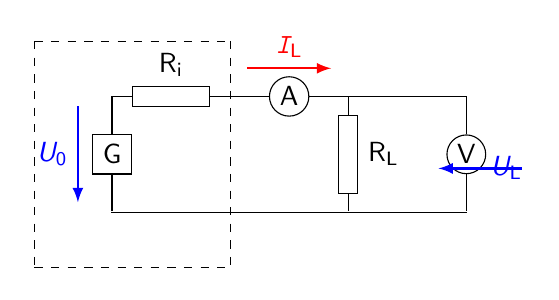
\begin{tikzpicture}[%show background rectangle,
circuit ee IEC, circuit symbol lines/.style={draw,thick},
font=\sffamily\upshape,
>=latex % Voreinstellung für Pfeilspitzen
]
\matrix (S) [
  matrix of nodes, nodes in empty cells,
  inner sep=0pt, outer sep=-.5\pgflinewidth,
  column sep=15mm, row sep = 7mm,
  nodes={minimum width=0pt}
  ]
{
  &&&  \\
  &&&  \\
  &&&  \\
  &&&  \\
};
 
 
%Orientierungshilfen
%\foreach \j in {1,...,3}
%{
%	\foreach \k in {1,...,4}
%	{%
%		\node[text=lightgray] at (S-\j-\k){+}; % Orientierungshilfe +
%		\node[red, left] at (S-\j-1){\j}; %Orientierungshilfe Zeilennummer
%		\node[red, above] at (S-1-\k){\k}; %Orientierungshilfe Spaltennummer  
%	};%
%}

%Bauteile
\draw (S-3-1) to  [generator={name=Gen}](S-1-1);

\draw (S-1-1) to  [resistor={info=R$_\mathsf{i}$, name=Wstd}](S-1-2);

\draw (S-1-3) to  [resistor={info=R$_\mathsf{L}$, name=Wstd1}](S-3-3);
\draw (S-1-4) to  [voltmeter ={name=VM1}](S-3-4);


\draw (S-1-2) to  [ammeter ={name=AM1}](S-1-3);

%Spannungspfeile
%Spannungspfeil der Quelle / des Voltmeters
\draw[UPfeil=-1em]([xshift=-.5em]Gen.north west) -- node [left]{U$\mathsf{_0}$}([xshift=-.5em]Gen.south west);
\draw[UPfeil=-1em]([xshift=.5em]VM1.north east) -- node [right]{U$\mathsf{_L}$}([xshift=.5em]VM1.south east);


%Strompfeile
\draw[IPfeil=-1em]([yshift=.5em]AM1.north west) -- node [above]{I$\mathsf{_L}$}([yshift=.5em]AM1.north east);

 
%Leiterbahnen

\draw (S-1-3) -- (S-1-4);
\draw (S-3-1) -- (S-3-4);

\draw [dashed]([xshift=-2.8em, yshift=2em]S-1-1.center) -- ([yshift=2em]S-1-2.center);

\draw [dashed]([xshift=-2.8em, yshift=2em]S-1-1.center) -- ([xshift=-2.8em, yshift=-2em]S-3-1.center);
\draw [dashed]([yshift=2em]S-1-2.center) -- ([yshift=-2em]S-3-2.center); 

\draw [dashed]([xshift=-2.8em, yshift=-2em]S-3-1.center) -- ([yshift=-2em]S-3-2.center); 
 
\end{tikzpicture}
\end{center}

\subsection{Aufbau der Schaltung}

In der oben skizzierten Schaltung ist aus dem Generator $G$ und dem Widerstand $R_i$, einem Lastwiderstand mit $100\Omega/10W$ eine Spannungsquelle aufgebaut.
Die Spannungsquelle wird mit mehreren den Belastungswiderständen zwischen $1\Omega$ und $10k\Omega$ belastet.

\newpage
\subsection{Messung der Spannung bei verschiedenen Belastungsfällen}

In einem ersten Messdurchgang wird die Ausgangsspannung $U_L$ für die Belastungsfälle zwischen $1\Omega$ und $10k\Omega$ gemessen.

\begin{flushleft}
\begin{tabular}{ l | c | c | c | c | c | c | c | c | c  }
    \hline
    $R_L$ in V  & 1    & 10   & 33   & 56   & 82   & 100  & 120  & 150  & 330         \\ \hline
    $U_L$ in V  & 0,1  & 0,88 & 2,43 & 3,49 & 4,22 & 4,91 & 5,35 & 5,91 & 7,67      \\
    \hline
\end{tabular} \\
\begin{tabular}{ l | c | c | c | c | c | c | c | c }
    \hline
    $R_L$ in V  & 560  & 820  & 1000  & 1500 & 3300 & 5600  & 8200  & 10000   \\ \hline
    $U_L$ in V  & 8,48 & 8,92 & 9,12  & 9,38 & 9,76 & 9,86  & 9,93  & 9,96    \\
    \hline
\end{tabular}
\end{flushleft}

\subsection{Grafische Darstellung}
Werden die Widerstandswerte im logarithmischen Maßstab aufgetragen lassen sich die Messwerte als Diagramm darstellen.

\begin{figure}[hbtp]
\centering
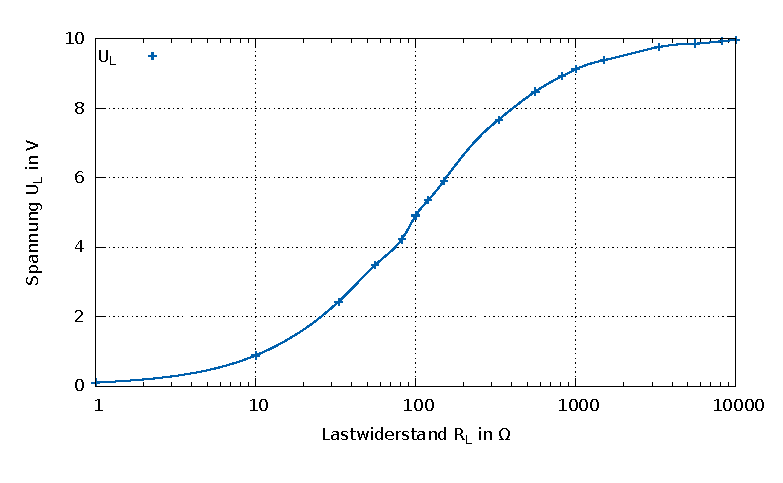
\includegraphics[scale=1]{diagramm_spannung.eps}
\end{figure}

\subsection{Grenzfälle}

Bei einem Lastwiderstand von $R_1=0\Omega$, der einem Kurzschluss der Spannungsquelle gleichkommt wird der Strom nur von dem Innenwiderstand der Spannungsquelle, hier $R_i=100\Omega$ begrenzt. Dementsprechend kann maximal ein Strom von $I_L=\frac{U_0}{R_i}=\frac{10V}{100\Omega}=100mA$ fließen. Die gemessene Ausgangsspannung $U_A$ bricht auf 0V zusammen. Ein Lastwiderstand von $R_L=\infty \Omega$ kommt einem offenen Stromkreis gleich. Es fließt kein strom und die gemessene Ausgangsspannung bleibt bei 10V

\section{Stromabhängigkeit}
\subsection{Messung der Spannung bei verschiedenen Belastungsfällen}

Im zweiten Messdurchgang werden die Stromwerte für den Parameter $I_L$ gemessen und die Tabelle erweitert.

\begin{flushleft}
\begin{tabular}{ l | c | c | c | c | c | c | c | c | c  }
    \hline
    $R_L$ in V   & 1    & 10   & 33   & 56   & 82   & 100  & 120  & 150  & 330         \\ \hline
    $U_L$ in V   & 0,1  & 0,88 & 2,43 & 3,49 & 4,22 & 4,91 & 5,35 & 5,91 & 7,67      \\ \hline
    $I_L$ in mA  & 95   & 88   & 73   & 63   & 54   & 49,5 & 45,5 & 40   & 23      \\
    \hline
\end{tabular} \\
\begin{tabular}{ l | c | c | c | c | c | c | c | c }
    \hline
    $R_L$ in V   & 560  & 820  & 1000  & 1500 & 3300 & 5600  & 8200  & 10.000   \\ \hline
    $U_L$ in V   & 8,48 & 8,92 & 9,12  & 9,38 & 9,76 & 9,86  & 9,93  & 9,96    \\ \hline
    $I_L$ in mA  & 15   & 11   & 9,1   & 6,3  & 2,95 & 1,75  & 1,2   & 0,99    \\
    \hline
\end{tabular}
\end{flushleft}
Mit den gemessenen Werten kann man das vorhin erstellte Diagramm um eine Stromkurve erweitern.
\begin{figure}[hbtp]
\centering
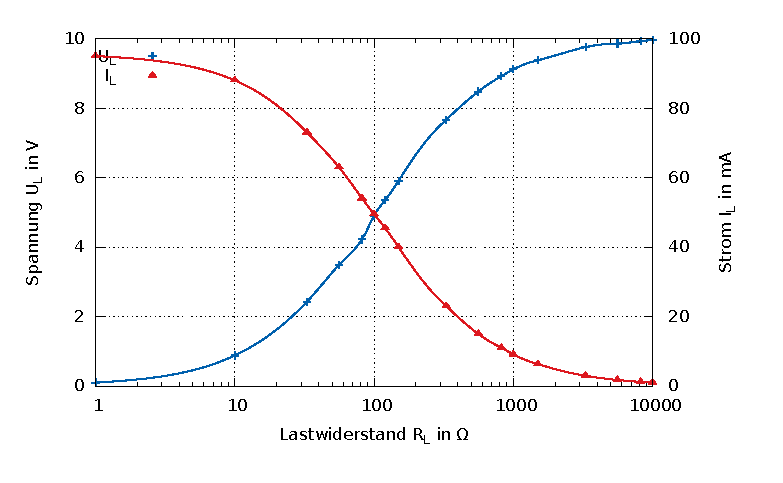
\includegraphics[scale=1]{diagramm_spannung_strom.eps}
\end{figure}


\section{Leistungsabhängigkeit}
\subsection{Leistung in allen Belastungsfällen}
Die elektrische Leistung, die im Lastwiderstand in Wärme umgesetzt wird, errechnet sich aus $P_{el}=U_{L} \cdot I_L$.


\begin{flushleft}
\begin{tabular}{ l | c | c | c | c | c | c | c | c | c  }
    \hline
    $R_L$ in V   & 1    & 10    & 33     & 56     & 82     & 100    & 120    & 150   & 330         \\ \hline
    $U_L$ in V   & 0,1  & 0,88  & 2,43   & 3,49   & 4,22   & 4,91   & 5,35   & 5,91  & 7,67      \\ \hline
    $I_L$ in mA  & 95   & 88    & 73     & 63     & 54     & 49,5   & 45,5   & 40    & 23      \\ \hline
    $P$ in mW    & 9,5  & 77,44 & 177,39 & 219,87 & 238,86 & 243,04 & 243,42 & 236,4 & 176,41      \\ 
    \hline
\end{tabular} \\
\begin{tabular}{ l | c | c | c | c | c | c | c | c }
    \hline
    $R_L$ in V  & 560    & 820   & 1000   & 1500  & 3300  & 5600   & 8200   & 10.000   \\ \hline
    $U_L$ in V  & 8,48   & 8,92  & 9,12   & 9,38  & 9,76  & 9,86   & 9,93   & 9,96    \\ \hline
    $I_L$ in mA & 15     & 11    & 9,1    & 6,3   & 2,95  & 1,75   & 1,2    & 0,99    \\ \hline
    $P$ in mW   & 127,2  & 98,12 & 82,99  & 59,09 & 28,79 & 17,25  & 11,91  & 9,86    \\
    \hline
\end{tabular}
\end{flushleft}
\subsection{Grafische Darstellung}
Mit den gemessenen Werten kann man das vorhin erstellte Diagramm um eine Stromkurve erweitern, sodass nun alle drei Kennlinien überlagert sind.

\begin{figure}[hbtp]
\centering
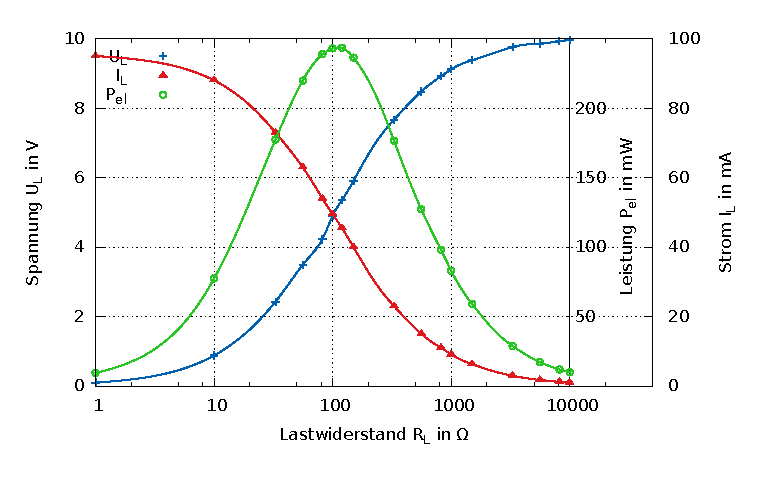
\includegraphics[scale=1]{diagramme.eps}
\end{figure}

\subsection{Grenzfälle der Leistung}
\textbf{blub blub, hier muss noch text hin}


\section{Erkenntnisse}
\textbf{blub blub, hier muss noch text hin}

%%%
%%% end main document
%%%
%%%%%%%%%%%%%%%%%%%%%%%%%%%%%%%%%%%%%%%%%%%%%%%%%%%%%%%%%%%%%%%%%%%%%%%%%%%%%%%%

% \appendix  %% include it, if something (bibliography, index, ...) follows below

%%%%%%%%%%%%%%%%%%%%%%%%%%%%%%%%%%%%%%%%%%%%%%%%%%%%%%%%%%%%%%%%%%%%%%%%%%%%%%%%
%%%
%%% bibliography
%%%
%%% available styles: abbrv, acm, alpha, apalike, ieeetr, plain, siam, unsrt
%%%
% \bibliographystyle{plain}

%%% name of the bibliography file without .bib
%%% e.g.: literatur.bib -> \bibliography{literatur}
% \bibliography{FIXXME}

\end{document}
%%% }}}
%%% END OF FILE
%%%%%%%%%%%%%%%%%%%%%%%%%%%%%%%%%%%%%%%%%%%%%%%%%%%%%%%%%%%%%%%%%%%%%%%%%%%%%%%%
%%% Notice!
%%% This file uses the outline-mode of emacs and the foldmethod of Vim.
%%% Press 'zi' to unfold the file in Vim.
%%% See ':help folding' for more information.
%%%%%%%%%%%%%%%%%%%%%%%%%%%%%%%%%%%%%%%%%%%%%%%%%%%%%%%%%%%%%%%%%%%%%%%%%%%%%%%%
%% Local Variables:
%% mode: outline-minor
%% OPToutline-regexp: "%% .*"
%% OPTeval: (hide-body)
%% emerge-set-combine-versions-template: "%a\n%b\n"
%% End:
%% vim:foldmethod=marker
